\clearpage
\section{Results}\label{sec:results}

\subsection{Coverage and quantitative comparison}
The main run contains all 99 configured combinations: eleven tasks times nine models. All completed successfully, including every one of the 321 ECL and 862 Traffic series. The 723,600 saved forecast rows contain no duplicate task/model/series/step keys or nonfinite targets or predictions. Recalculation reproduces all four metrics in 99 overall, 15,012 per-series and 5,184 per-horizon rows. The TimesFM study similarly contains 44 successful combinations and 237,072 forecast rows. These checks establish internal consistency of saved results; they are not independent executions of the forecasting models.

Tables~\ref{tab:smape1}--\ref{tab:mase2} contain the complete task--model comparison. Appendix~\ref{sec:fullscores} supplies all MAE and RMSE scores. The panels are intentionally kept separate because their units and forecast durations differ. Foundation models are often competitive, but their advantage is neither universal nor invariant to the metric.

\begin{table}[!htbp]
\centering
\caption{sMAPE by task, part 1 ($\downarrow$). Bold: minimum before rounding; exact ties share bold. Bolt denotes Chronos-Bolt; SNaive denotes SeasonalNaive.}
\label{tab:smape1}
\small
\setlength{\tabcolsep}{3.5pt}
\begin{tabular}{lrrrrrrrrr}
\hline
Task & Linear & TabPFN & TimesFM & Bolt & Prophet & ARIMA & ETS & Theta & SNaive \\
\hline
M4 Hourly & 31.86 & 14.49 & 8.61 & \textbf{8.35} & 18.06 & 41.27 & 17.19 & 18.16 & 13.91 \\
ETTh1/48 & 48.18 & 51.14 & 32.96 & 32.80 & 64.91 & 38.82 & 38.87 & 70.43 & \textbf{23.21} \\
ETTh1/96 & 52.27 & 49.51 & 43.00 & 40.20 & 63.59 & 41.35 & 42.65 & 67.52 & \textbf{34.82} \\
ETTh2/48 & 23.14 & 27.82 & 24.90 & 25.00 & 51.61 & \textbf{18.39} & 18.74 & 21.33 & 20.14 \\
ETTm1/48 & 53.11 & 42.30 & 35.69 & 37.23 & 76.84 & 42.29 & 55.48 & 60.73 & \textbf{31.06} \\
ETTm2/48 & 9.30 & 9.69 & 5.46 & 7.01 & 22.80 & 5.26 & \textbf{4.81} & 8.71 & 15.68 \\
\hline
\end{tabular}
\end{table}

\begin{table}[!htbp]
\centering
\caption{sMAPE by task, part 2 ($\downarrow$). Bold: minimum before rounding; exact ties share bold. Bolt denotes Chronos-Bolt; SNaive denotes SeasonalNaive.}
\label{tab:smape2}
\small
\setlength{\tabcolsep}{3.5pt}
\begin{tabular}{lrrrrrrrrr}
\hline
Task & Linear & TabPFN & TimesFM & Bolt & Prophet & ARIMA & ETS & Theta & SNaive \\
\hline
ECL & 27.99 & 19.95 & 14.17 & \textbf{11.43} & 23.31 & 51.93 & 16.44 & 19.91 & 14.02 \\
Traffic & 48.74 & 44.68 & 32.71 & \textbf{25.35} & 64.13 & 72.96 & 68.89 & 46.91 & 31.49 \\
Weather & 76.82 & 60.76 & 39.88 & \textbf{19.53} & 34.74 & 54.94 & 30.57 & 44.73 & 22.02 \\
Exchange & \textbf{1.85} & 2.28 & 2.11 & 2.30 & 4.56 & 2.11 & 2.07 & 2.23 & 2.71 \\
ILI & 73.53 & 59.85 & \textbf{16.21} & 63.11 & 73.04 & 41.60 & 30.76 & 48.59 & 62.34 \\
\hline
\end{tabular}
\end{table}

\begin{table}[!htbp]
\centering
\caption{MASE by task, part 1 ($\downarrow$). Bold: minimum before rounding; exact ties share bold. Bolt denotes Chronos-Bolt; SNaive denotes SeasonalNaive.}
\label{tab:mase1}
\small
\setlength{\tabcolsep}{3.5pt}
\begin{tabular}{lrrrrrrrrr}
\hline
Task & Linear & TabPFN & TimesFM & Bolt & Prophet & ARIMA & ETS & Theta & SNaive \\
\hline
M4 Hourly & 9.488 & 1.684 & \textbf{0.734} & 0.835 & 1.626 & 16.922 & 1.606 & 2.456 & 1.193 \\
ETTh1/48 & 1.062 & 1.094 & 0.568 & 0.606 & 1.357 & 0.752 & 0.757 & 1.349 & \textbf{0.367} \\
ETTh1/96 & 1.248 & 1.103 & 0.904 & 0.845 & 1.399 & 0.980 & 1.026 & 1.394 & \textbf{0.720} \\
ETTh2/48 & 0.684 & 0.718 & 0.665 & 0.604 & 1.257 & 0.595 & \textbf{0.590} & 0.689 & 0.620 \\
ETTm1/48 & 1.028 & 0.723 & 0.457 & 0.432 & 1.367 & 0.923 & 1.087 & 0.951 & \textbf{0.394} \\
ETTm2/48 & 0.425 & 0.453 & 0.278 & 0.312 & 1.269 & 0.283 & \textbf{0.270} & 0.429 & 0.628 \\
\hline
\end{tabular}
\end{table}

\begin{table}[!htbp]
\centering
\caption{MASE by task, part 2 ($\downarrow$). Bold: minimum before rounding; exact ties share bold. Bolt denotes Chronos-Bolt; SNaive denotes SeasonalNaive.}
\label{tab:mase2}
\small
\setlength{\tabcolsep}{3.5pt}
\begin{tabular}{lrrrrrrrrr}
\hline
Task & Linear & TabPFN & TimesFM & Bolt & Prophet & ARIMA & ETS & Theta & SNaive \\
\hline
ECL & 2.645 & 1.735 & 1.294 & \textbf{1.028} & 1.823 & 5.020 & 1.483 & 1.998 & 1.405 \\
Traffic & 1.188 & 1.078 & 0.648 & \textbf{0.604} & 1.429 & 1.957 & 1.563 & 1.443 & 0.869 \\
Weather & 3.605 & 0.213 & \textbf{0.118} & 0.132 & 0.444 & 0.190 & 0.176 & 0.142 & 0.298 \\
Exchange & \textbf{5.560} & 7.422 & 6.928 & 6.564 & 14.571 & 7.446 & 6.720 & 7.935 & 8.779 \\
ILI & 3.540 & 3.714 & \textbf{0.605} & 3.231 & 3.393 & 2.080 & 2.013 & 2.349 & 3.783 \\
\hline
\end{tabular}
\end{table}


On M4 Hourly, Chronos-Bolt has the lowest sMAPE (8.35 versus TimesFM's 8.61), whereas TimesFM has the lowest MASE (0.734 versus 0.835). ECL and Traffic favour Bolt on both metrics. For Traffic, its sMAPE of 25.35 is below SeasonalNaive's 31.49 and TimesFM's 32.71; nevertheless TimesFM's MASE of 0.648 is below SeasonalNaive's 0.869. These comparisons show that percentage error and train-scaled absolute error can assign different importance to the same series and observations.

ETT provides counterexamples to an unconditional foundation-model advantage. SeasonalNaive is best on both metrics for ETTh1/48, ETTh1/96 and ETTm1/48. For ETTh1/48 its sMAPE is 23.21, compared with 32.96 for TimesFM, and its MASE is 0.367 versus 0.568. At ETTh1/96 the errors increase for all three of SeasonalNaive, TimesFM and Bolt. This is not a controlled horizon-only comparison: the origin is also moved 48 observations earlier and the training period changes. AutoARIMA is best by sMAPE on ETTh2/48, while AutoETS is best by MASE there and by both metrics on ETTm2/48.

Weather is especially sensitive to the metric: Bolt's sMAPE is 19.53, SeasonalNaive's 22.02 and TimesFM's 39.88, but TimesFM attains the lowest MASE, 0.118. This apparent reversal is compatible with a mixture of physical units, near-zero targets and distinct train-derived scales; the qualitative examples below inspect one such case. On Exchange, linear regression is best on both metrics. Even its MASE of 5.560 exceeds one, despite sMAPE of only 1.85, illustrating how a small percentage error can still be large relative to typical lag-one training changes. On ILI, TimesFM leads strongly: 16.21 sMAPE and 0.605 MASE, compared with the next-best sMAPE of 30.76 for AutoETS. The seven related surveillance variables do not constitute seven independent replications of that advantage.

Prophet completes every task but is never best in these overall tables. Its sMAPE is 18.06 on M4, 64.91 on ETTh1/48 and 73.04 on ILI. On Weather it improves on TimesFM by sMAPE (34.74 versus 39.88), while performing substantially worse by MASE (0.444 versus 0.118). The automatic fitting setup, limited histories and absence of application-specific calendar adjustments constrain interpretation. The results assess this configuration of Prophet, not the full range of analyst-specified models that it supports. TabPFN likewise has no overall minimum in either metric, but improves on the common linear representation on M4, ECL and Traffic. Its weaker results elsewhere cannot establish the performance of published TabPFN-TS, whose adaptation is different.

\subsection{Error across the forecast horizon}\label{sec:horizonresults}
Figure~\ref{fig:horizons} displays selected sMAPE profiles for M4, ETTh1/96, Traffic and Weather, with corresponding MASE profiles in Appendix~\ref{sec:fullscores}. Each point aggregates the same series at a different step of the same held-out trajectories. The curves are not repeated independent experiments, and a local peak can reflect the values or seasonal phase encountered at that step. Accordingly they should not be interpreted as confidence bands or as an estimate averaged over random forecast origins. The task-level metrics summarize the entire curves; selecting only a favourable prefix would change the evaluation question.

The profiles are visibly non-monotone. On M4, TimesFM and Bolt remain close while Prophet and SeasonalNaive show larger excursions. ETTh1/96 has recurring peaks and troughs across the four-day continuation, with Prophet often above the other displayed curves. Traffic shows a pronounced late rise for Prophet, while Weather has comparatively irregular TimesFM percentage errors and a generally lower Bolt curve. These patterns localize the aggregate differences without establishing a universal relationship between horizon length and error.

\begin{figure}[!htbp]\centering
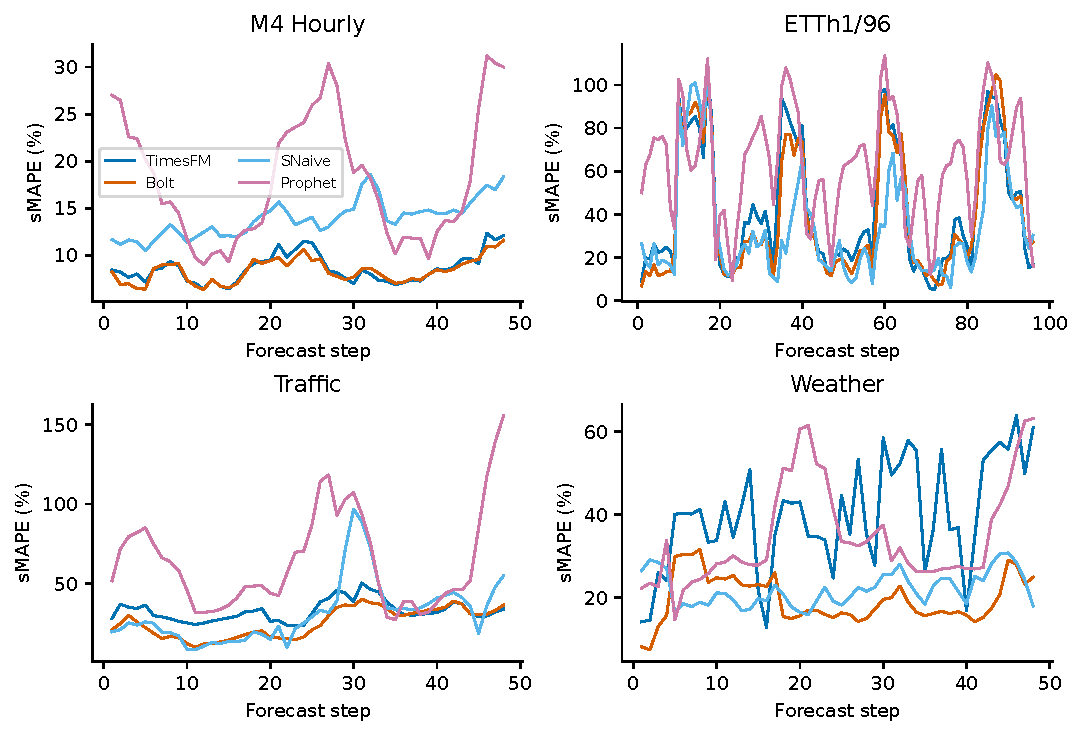
\includegraphics[width=\linewidth]{img/experiments/horizon_smape.pdf}
\caption{Per-step sMAPE of four selected comparators. All models' complete overall scores are given in the preceding tables.}\label{fig:horizons}
\end{figure}

\subsection{Observed histories and forecast continuations}\label{sec:qualitative}
Six diagnostic examples are selected from saved predictions. Within a task, series are sorted by TimesFM test sMAPE, with string ID breaking ties; ``median'' means the middle sorted series (upper middle for an even count). M4 contributes its best and worst series, ETTh1 and Traffic their median series, Weather its worst and ILI its median. This is deliberate selection using test errors, not a random representative sample. Table~\ref{tab:selections} discloses the IDs and all displayed per-series scores. Four model curves retain visibility while including Prophet. Each plot contains at least three nominal seasonal cycles or twice the horizon in training history, whichever is larger; zero marks the final training observation, and the black line is the actual continuation.

\begin{table}[!htbp]
\centering
\caption{Diagnostic examples ranked by TimesFM test sMAPE; all entries are per-series sMAPE ($\downarrow$). Median means the middle sorted series (upper middle for even counts).}
\label{tab:selections}
\small
\setlength{\tabcolsep}{3.5pt}
\begin{tabular}{lrrrrrr}
\hline
Task & ID & Rule & TimesFM & Bolt & SNaive & Prophet \\
\hline
M4 Hourly & H187 & best & 0.15 & 0.27 & 0.09 & 0.31 \\
M4 Hourly & H349 & worst & 84.71 & 85.46 & 83.01 & 102.42 \\
ETTh1/48 & HUFL & median & 26.54 & 40.36 & 8.89 & 71.84 \\
Traffic & 193 & median & 18.65 & 15.63 & 20.07 & 80.54 \\
Weather & max. PAR & worst & 158.46 & 187.96 & 3.79 & 41.27 \\
ILI & AGE 5-24 & median & 9.95 & 74.00 & 83.95 & 112.74 \\
\hline
\end{tabular}
\end{table}


\begin{figure}[p]\centering
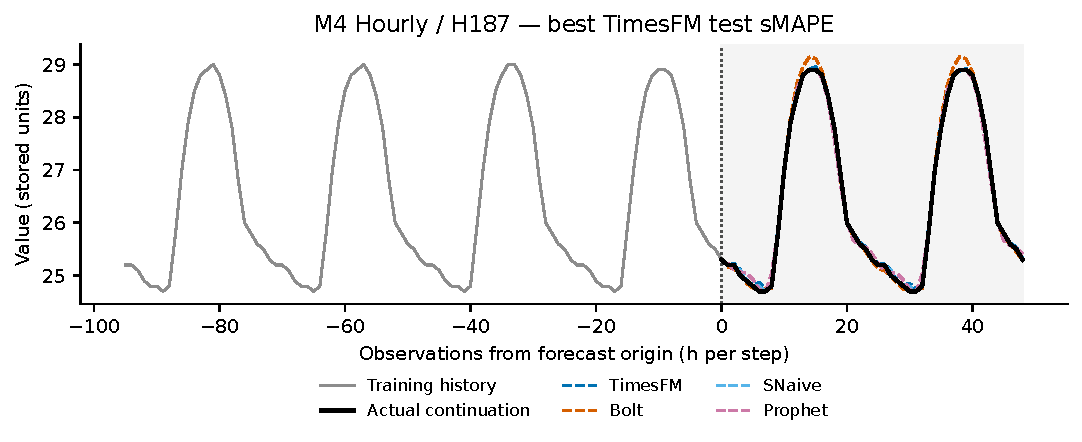
\includegraphics[width=\linewidth]{img/experiments/forecast_1.pdf}
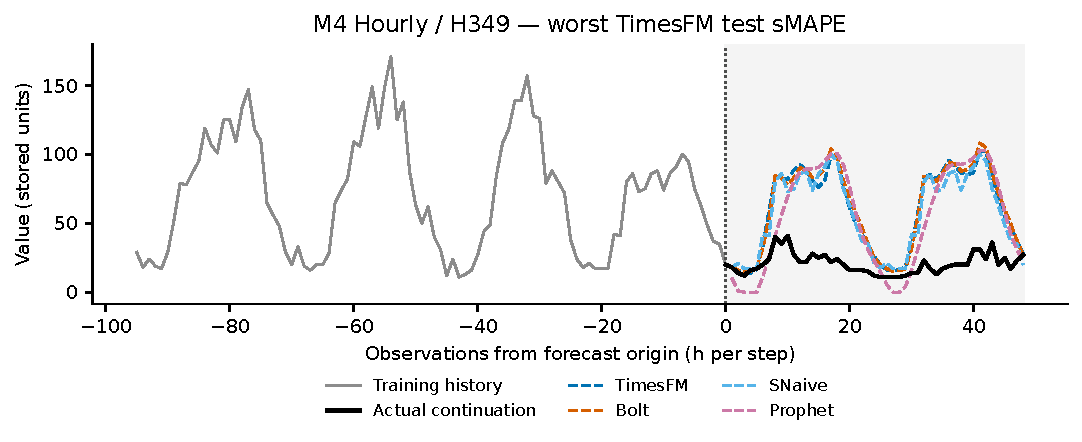
\includegraphics[width=\linewidth]{img/experiments/forecast_2.pdf}
\caption{M4 Hourly: H187 (best TimesFM test sMAPE; rank 1/414) and H349 (worst; rank 414/414). Origins are integer position 960, with 96 historical observations shown. The examples expose both a predictable continuation and a continuation with much smaller peaks than the recent history.}\label{fig:m4examples}
\end{figure}

In H187, low TimesFM error does not imply that TimesFM is the best model: SeasonalNaive obtains 0.087 sMAPE compared with 0.149 for TimesFM. At the other extreme, H349's actual test peaks are much smaller than its recent historical peaks. All four displayed methods extrapolate larger recurring peaks and incur high error; TimesFM's sMAPE is 84.71 and Prophet's 102.42. This is evidence of a failure on this continuation, not proof of a particular unobserved intervention or regime-change mechanism.

\begin{figure}[p]\centering
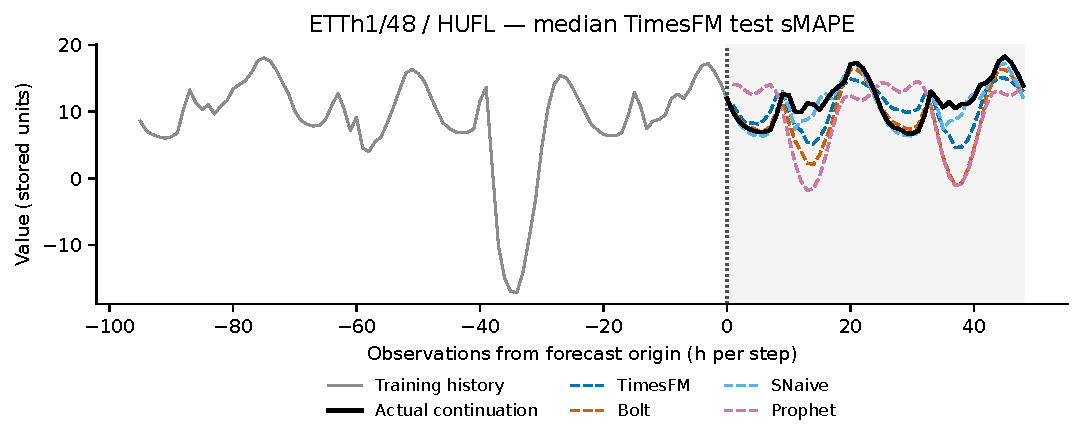
\includegraphics[width=\linewidth]{img/experiments/forecast_3.pdf}
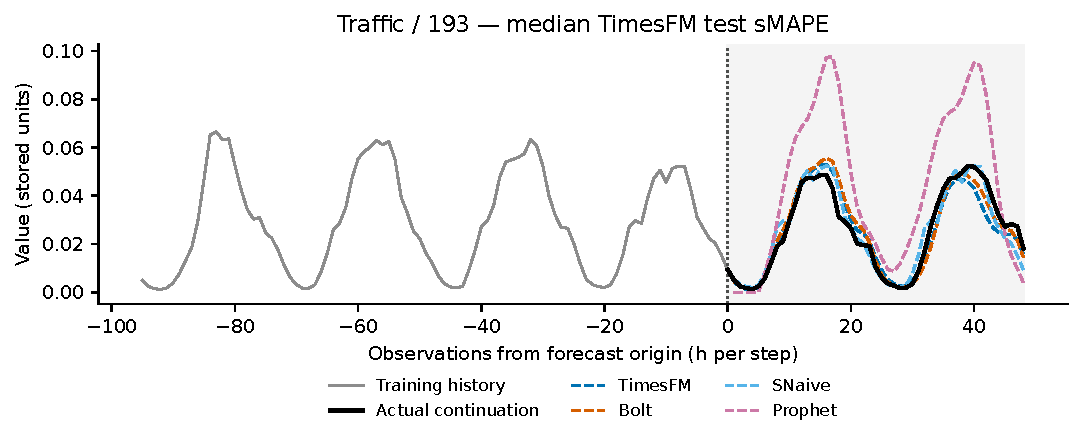
\includegraphics[width=\linewidth]{img/experiments/forecast_4.pdf}
\caption{ETTh1/48: HUFL (rank 4/7), origin 2018-02-18 23:00; Traffic: ID 193 (rank 432/862), archive origin 2018-06-30 01:00. Both show 96 historical observations. TimesFM is the reference for selection, regardless of which comparator performs best.}\label{fig:ettexamples}
\end{figure}

ETTh1 HUFL is a clear counterexample: SeasonalNaive follows the repeated daily continuation more closely (8.89 sMAPE) than TimesFM (26.54), Bolt (40.36) or Prophet (71.84). Traffic ID 193 instead favours Bolt (15.63), followed by TimesFM (18.65) and SeasonalNaive (20.07), while Prophet has 80.54. The examples demonstrate why a diagnostic figure should show actual values and temporal alignment, rather than only aggregate error.

\begin{figure}[p]\centering
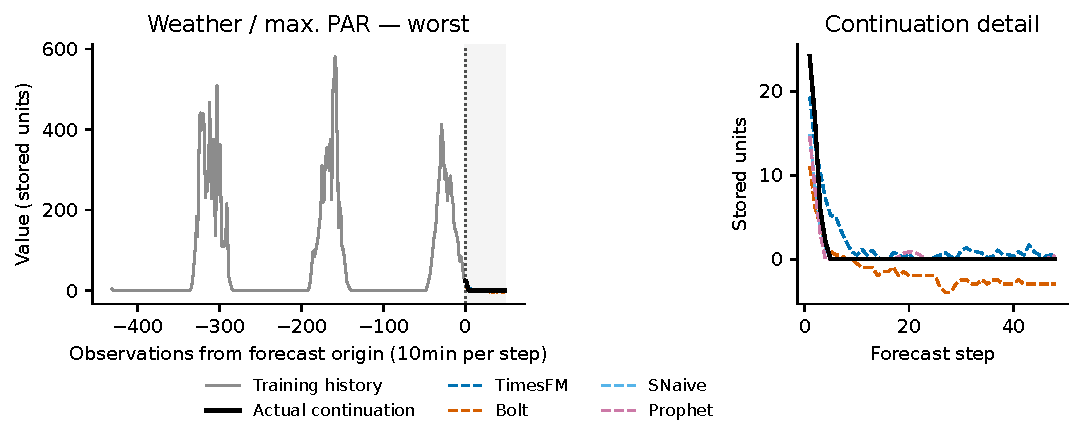
\includegraphics[width=\linewidth]{img/experiments/forecast_5.pdf}
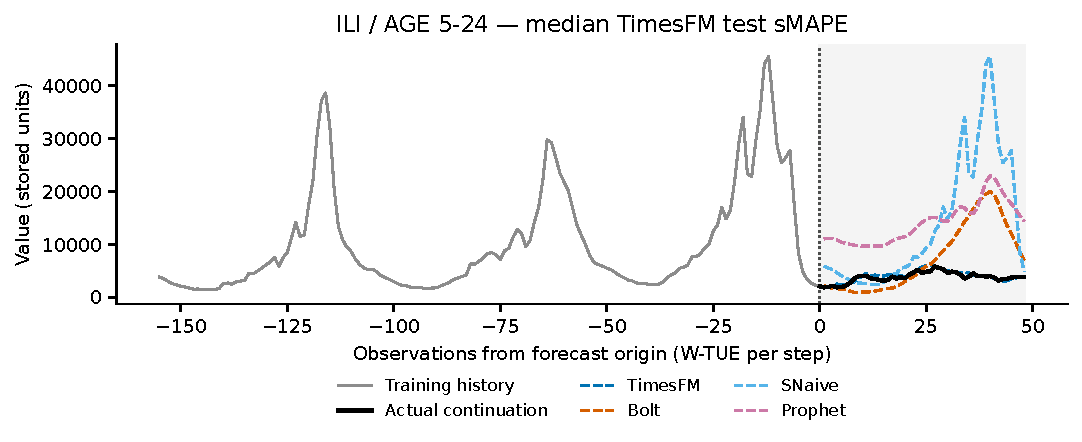
\includegraphics[width=\linewidth]{img/experiments/forecast_6.pdf}
\caption{Weather: maximum PAR (rank 21/21), origin 2020-12-31 16:00, 432 training observations; the right panel enlarges the continuation. ILI: AGE 5--24 (rank 4/7), archive origin 2019-07-30, 156 training observations. The Weather header's damaged unit characters are omitted in the display ID; the exact stored ID is preserved in the evidence manifest.}\label{fig:weatheriliexamples}
\end{figure}

The Weather maximum-PAR example has a near-zero evening continuation after pronounced daytime peaks. SeasonalNaive obtains 3.79 sMAPE; TimesFM and Bolt obtain 158.46 and 187.96. The enlarged continuation makes visible discrepancies that are barely visible on the historical amplitude scale. This does not contradict small absolute errors on other variables, nor TimesFM's leading overall Weather MASE. On ILI AGE 5--24 the actual continuation remains much lower than the strongest preceding seasonal peaks. TimesFM follows that lower trajectory more closely (9.95 sMAPE), while Bolt, SeasonalNaive and Prophet obtain 74.00, 83.95 and 112.74. Because the archive's surveillance-date mapping is not verified, no particular public-health event is assigned as the cause.

\clearpage
\subsection{Characteristics associated with error}\label{sec:correlations}
The analysis contains 1,668 task--series entries and 15,012 feature--model rows. ETTh1 appears at two horizons, and most entries come from Traffic, M4 and ECL. Tables~\ref{tab:corrsmape} and \ref{tab:corrmase} focus on those three larger panels, using seasonal ACF and STL seasonal strength rather than selecting correlations by statistical significance. Figure~\ref{fig:features} shows the individual TimesFM observations. ECL contributes 320 valid pairs, since ID 182 has an all-zero final 10,000-observation tail and hence undefined ACF and STL strengths; its full training MASE denominator is nonetheless positive.

\begin{table}[!htbp]
\centering
\caption{Within-task Spearman correlations with per-series sMAPE. $n$ is the valid-pair count for each displayed model. }
\label{tab:corrsmape}
\small
\setlength{\tabcolsep}{3.5pt}
\begin{tabular}{lrrrrr}
\hline
Task & Feature & $n$ & TimesFM & Bolt & SNaive \\
\hline
M4 Hourly & ACF($s$) & 414 & -0.827 & -0.827 & -0.832 \\
M4 Hourly & STL seasonal & 414 & -0.859 & -0.858 & -0.860 \\
ECL & ACF($s$) & 320 & -0.084 & -0.079 & -0.156 \\
ECL & STL seasonal & 320 & -0.056 & -0.067 & -0.137 \\
Traffic & ACF($s$) & 862 & -0.072 & -0.075 & -0.111 \\
Traffic & STL seasonal & 862 & -0.144 & -0.130 & -0.174 \\
\hline
\end{tabular}
\end{table}

\begin{table}[!htbp]
\centering
\caption{Within-task Spearman correlations with per-series MASE. $n$ is the valid-pair count for each displayed model. The MASE view is an additional descriptive analysis of saved results.}
\label{tab:corrmase}
\small
\setlength{\tabcolsep}{3.5pt}
\begin{tabular}{lrrrrr}
\hline
Task & Feature & $n$ & TimesFM & Bolt & SNaive \\
\hline
M4 Hourly & ACF($s$) & 414 & 0.064 & 0.329 & 0.141 \\
M4 Hourly & STL seasonal & 414 & 0.031 & 0.305 & 0.114 \\
ECL & ACF($s$) & 320 & 0.446 & 0.373 & 0.418 \\
ECL & STL seasonal & 320 & 0.502 & 0.422 & 0.471 \\
Traffic & ACF($s$) & 862 & 0.129 & 0.108 & 0.095 \\
Traffic & STL seasonal & 862 & 0.116 & 0.108 & 0.093 \\
\hline
\end{tabular}
\end{table}


For M4, the association between seasonal regularity and sMAPE is strong and negative for all displayed models. TimesFM has $\rho=-0.827$ for seasonal ACF and $-0.859$ for STL strength, with comparable values for Bolt and SeasonalNaive. In ECL and Traffic, the corresponding TimesFM associations are much weaker: seasonal ACF gives $-0.084$ and $-0.072$. Thus the M4 pattern does not support a universal relationship of that magnitude across domains.

The additional MASE analysis changes this interpretation substantially. On M4, TimesFM's correlation with STL seasonal strength becomes 0.031; on ECL it becomes 0.502. MASE divides each series' error by its own training naive error, whereas sMAPE divides individual errors by target/prediction magnitudes. A relationship between seasonal structure and the MASE denominator can therefore contribute to the observed sign changes. This is a possible statistical explanation, not an experimentally established causal mechanism. The data support metric-specific associations, not a claim that increasing seasonality would improve or worsen a model's forecasts.

The small ETT and ILI panels each contain only seven related variables; Weather has 21 and Exchange eight. Their full descriptive correlations remain in the evidence package but do not justify population-level inference. Pooled correlations additionally combine frequencies, domains, repeated ETTh1 tasks and unequal panel sizes. Without uncertainty estimation or a dependence-aware sampling design, neither pooled nor within-panel coefficients establish significance, causal effects or a reliable rule for model selection.

\begin{figure}[!htbp]\centering
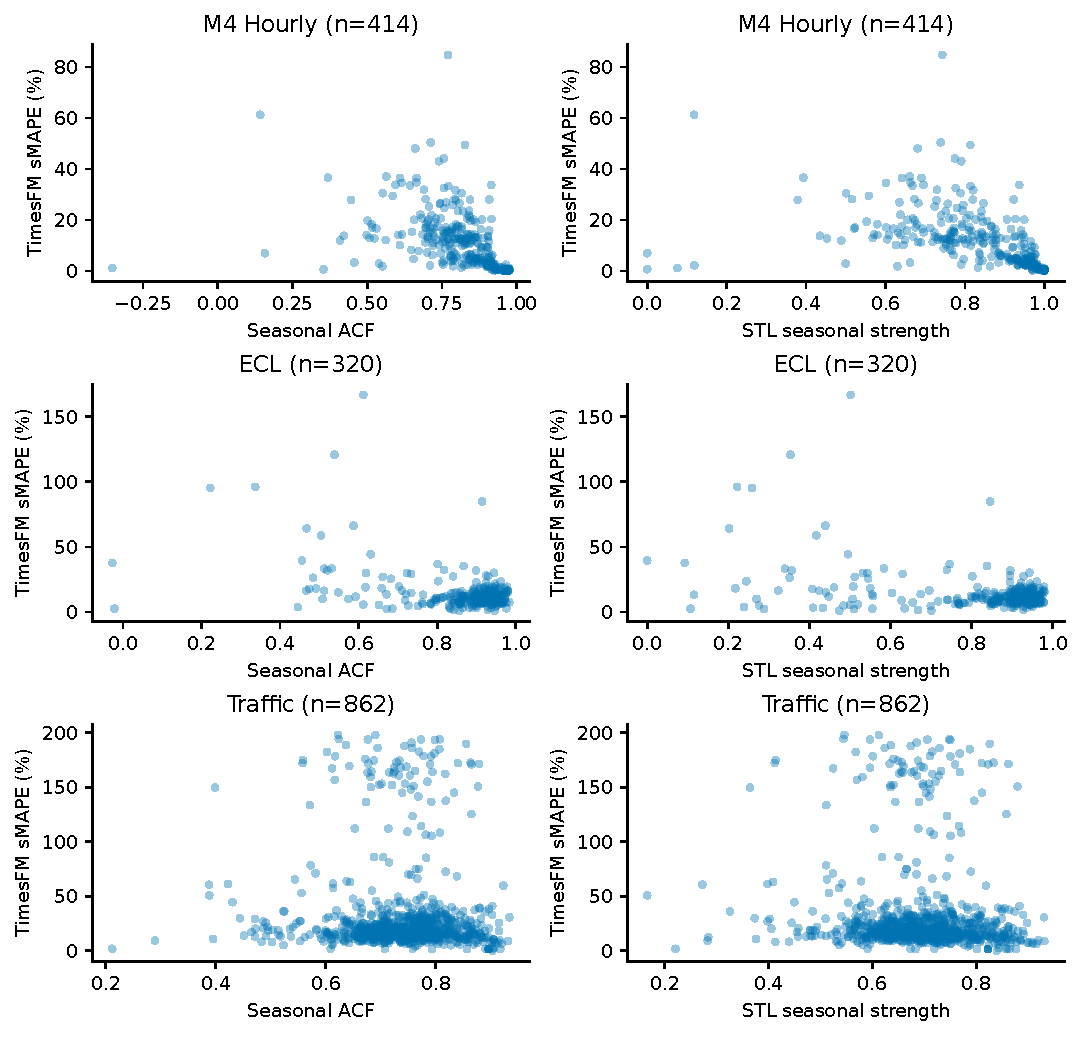
\includegraphics[width=.95\linewidth]{img/experiments/feature_scatter.pdf}
\caption{TimesFM per-series test sMAPE against train-only seasonal ACF and STL seasonal strength. Each point is one valid series-feature pair; axes and sample sizes differ across tasks.}\label{fig:features}
\end{figure}

\clearpage
\subsection{TimesFM sensitivity results}\label{sec:sensitivityresults}
Figure~\ref{fig:contexts} presents both sMAPE and MASE for every context setting; Appendix~\ref{sec:fullscores} tabulates the values. Larger context is not uniformly better. M4 changes from 8.664 sMAPE at 512 to 8.606 at 1,024 and remains unchanged at displayed precision for longer contexts. There are no additional real observations beyond 960, so this is effective-history saturation rather than evidence against the use of long context on longer series.

ETTh1 improves from 37.274 at 512 to 31.569 at 2,048, but reaches 33.920 at 16,256; its best observed context is 2,048 under both metrics. ETTm1 is best by sMAPE at 512 (35.345) but by MASE at 4,096 (0.4308). Weather reaches its lowest observed sMAPE at 8,192 (33.724), yet its lowest MASE at 4,096 (0.1148). These are descriptions of this test grid, not validation-based selections for deployment or unbiased improvements over the main comparison.

\begin{figure}[!htbp]\centering
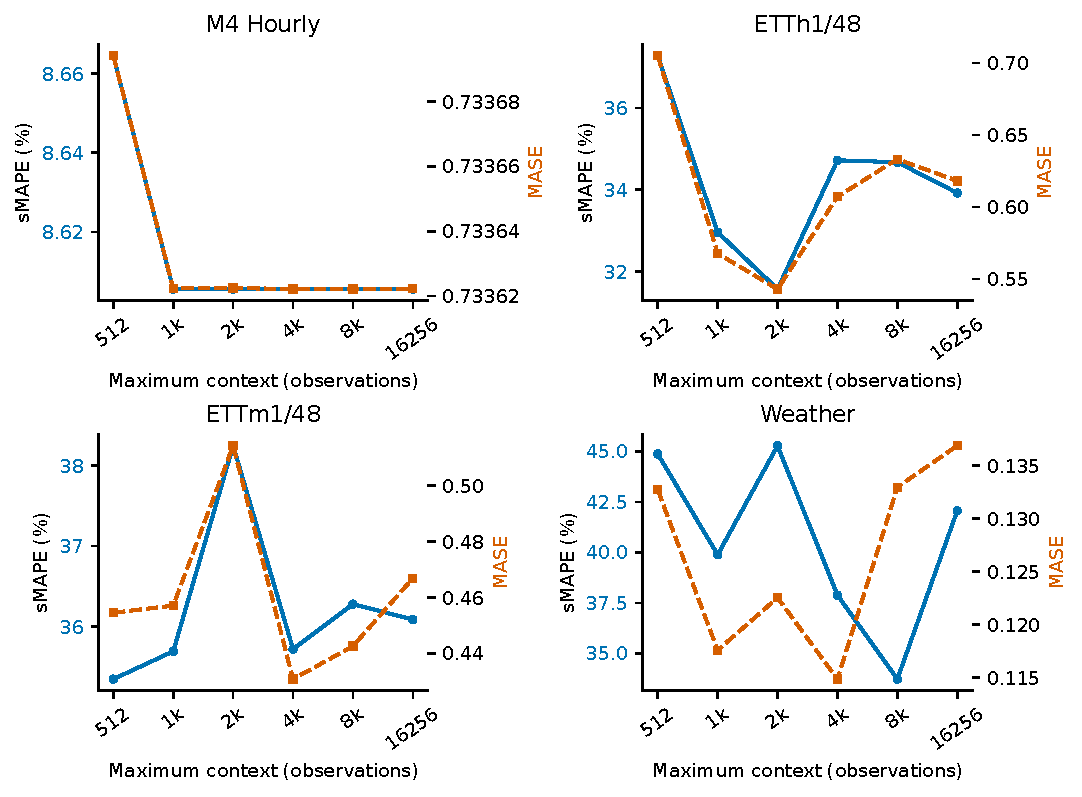
\includegraphics[width=\linewidth]{img/experiments/timesfm_context.pdf}
\caption{Context sensitivity with fixed checkpoint identifier. Blue circles use the left sMAPE axis; orange squares use the right MASE axis. The two vertical scales are independent. Grid positions are equally spaced categories, not a linear context-length scale.}\label{fig:contexts}
\end{figure}

\begin{table}[!htbp]
\centering
\caption{Change in sMAPE (percentage points) when the named flag is disabled, relative to the same-run 1,024-context baseline. Negative is better; rounded zeros can conceal small differences.}
\label{tab:flagssmape}
\small
\setlength{\tabcolsep}{3.5pt}
\begin{tabular}{lrrrr}
\hline
Disabled flag & M4 & ETTh1 & ETTm1 & Weather \\
\hline
Normalization & +0.000 & +0.000 & -0.000 & -0.000 \\
Quantile head & +0.000 & +0.000 & +0.000 & +0.000 \\
Flip invariance & +0.373 & +2.911 & -2.905 & -6.944 \\
Positive inference & +0.000 & +0.000 & +0.000 & +1.389 \\
Crossing repair & +0.000 & +0.000 & +0.000 & +0.000 \\
\hline
\end{tabular}
\end{table}

\begin{table}[!htbp]
\centering
\caption{Change in MASE when the named flag is disabled, relative to the same-run 1,024-context baseline. Negative is better; rounded zeros can conceal small differences.}
\label{tab:flagsmase}
\small
\setlength{\tabcolsep}{3.5pt}
\begin{tabular}{lrrrr}
\hline
Disabled flag & M4 & ETTh1 & ETTm1 & Weather \\
\hline
Normalization & -0.0000 & +0.0000 & -0.0000 & +0.0000 \\
Quantile head & +0.0000 & +0.0000 & +0.0000 & +0.0000 \\
Flip invariance & +0.0335 & +0.0483 & -0.0381 & +0.0023 \\
Positive inference & +0.0000 & +0.0000 & +0.0000 & +0.0000 \\
Crossing repair & +0.0000 & +0.0000 & +0.0000 & +0.0000 \\
\hline
\end{tabular}
\end{table}


Disabling flip invariance has the clearest nonzero effect. Relative to the common baseline, it raises sMAPE by 0.373 percentage points on M4 and 2.911 on ETTh1, but lowers it by 2.905 on ETTm1 and 6.944 on Weather. Weather again has a metric conflict: MASE increases by 0.0023. Disabling positive inference raises Weather sMAPE by 1.389 points but changes MASE by only about $1.31\times10^{-5}$, which rounds to zero in Table~\ref{tab:flagsmase}. The independent wrapper clipping still operates, so this is not a complete removal of positivity handling.

Disabling normalization produces absolute task-level sMAPE differences below $2\times10^{-6}$ points. Disabling the continuous quantile head or crossing repair produces exactly equal saved overall point scores in these tasks. The inspected point-return path uses the median channel, while these operations modify other quantile channels, providing an implementation-level explanation for the latter null effects. They do not test quantile quality or establish general irrelevance of those settings. The historical requested-versus-effective configuration limitation from Section~\ref{sec:sensitivity} also applies.

\subsection{Discussion, pretraining overlap and limitations}\label{sec:limitations}
The completed benchmark demonstrates substantial task and metric dependence. Bolt is strong on the large ECL and Traffic panels, TimesFM is strong on ILI and selected MASE comparisons, and simple or fitted statistical models lead several ETT tasks. Linear regression is competitive on Exchange. Neither architecture size nor pretraining alone explains the entire ranking, and the present design cannot identify which component causes a performance difference.

\paragraph{What zero-shot means here.}
TimesFM and Bolt undergo no target-data weight updates in this project. That operational fact does not establish that their pretrained checkpoints never saw these targets. The original TimesFM paper includes M4 in its training corpus~\cite{timesfm_paper}. The 2.5 card instead lists GiftEvalPretrain, Wikimedia Pageviews, Google Trends and synthetic/augmented data~\cite{timesfm_card}. These are version-specific disclosures; neither establishes exact exposure of this benchmark's final targets for the unpinned checkpoint used here.

The original Chronos paper separates M4 Hourly and Electricity Hourly as in-domain evaluation, while ETT and Traffic belong to its zero-shot partition. Its Weather entry is daily Australian weather, not the ten-minute Jena panel~\cite{chronos_paper}. The Bolt card explicitly claims no training exposure to its 27-dataset zero-shot benchmark~\cite{chronos_bolt_card}; this is relevant author-provided exclusion evidence, not an independent audit of the exact local arrays or checkpoint revision. No verified mapping establishes overlap or exclusion for every evaluated version, particularly renamed/relabelled Weather and ILI columns. TabPFN-TS describes synthetic tabular pretraining~\cite{tabpfn_ts}, but that paper does not identify the exact package-default weights used by this project's TabPFN 8.0.8. The appropriate conclusion is therefore pretrained inference with qualified provenance, rather than a blanket claim of either contamination or clean unseen-domain generalization.

\paragraph{Evaluation limits.}
One final origin can coincide with an unusually easy or difficult continuation. No sampling distribution for performance differences is estimated. Equal observation horizons represent radically different durations, and the repeated ETTh1 tasks overlap. ETT, Weather and ILI variables can be dependent. Large panels dominate pooled feature analyses, but not the task-separated result tables. Different history budgets, constrained AutoARIMA search, automatic Prophet settings, and a custom pooled TabPFN adaptation are additional comparison limits. Forecasts remain numerically reproducible from stored artifacts even though dirty source provenance and unpinned checkpoints prevent a claim of exact historical model reconstruction.

\paragraph{Extensions supported as future work.}
A validation period followed by a separate test would be needed to select contexts or flags. Multiple rolling origins and dependence-aware uncertainty estimates would be needed to assess stability of rankings. Equalized-history comparisons, broader statistical searches and a direct implementation of published TabPFN-TS would isolate adaptation and budget effects. Fine-tuning, XReg, probabilistic calibration and evaluation on independently verified unseen data are prospective experiments. None is necessary to describe the saved benchmark, and none is claimed as a completed contribution here.
